\documentclass{beamer}
\usepackage[utf8]{inputenc}
\usetheme{Antibes}
\usecolortheme{beaver}
\setbeamertemplate{navigation symbols}{}
\usepackage{amsmath, amssymb}
\usepackage{graphicx, tipa}
\usepackage{wrapfig}
\usepackage[export]{adjustbox}
\usepackage{float}
\newcommand{\arc}[1]{{%
		\setbox9=\hbox{#1}%
		\ooalign{\resizebox{\wd9}{\height}{\texttoptiebar{\phantom{A}}}\cr#1}}}

\title{Circle Geometry Lesson}
\author{SLSS Math Club 2019}
\date{April 17, 2019}

\begin{document}
\frame{\titlepage}

\section{Introduction}
	\begin{frame}{Introduction}
	\begin{itemize}
	    \item Circle geometry is an area of mathematics which involves geometry applied on a circle.
	    \item Many problems on the various mathematics contests, such as the Euclid, contain interesting and difficult circle geometry problems. 
	    \item Some elementary geometry knowledge such as properties of triangles, congruence and similarity, and properties of quadrilaterals are required as a prerequisite to this
topic.
\end{itemize}
\end{frame}
	
\section{Terminology}
\begin{frame}{Terminology}
\begin{itemize}
		\item Radius ($OA$): the segment between the center ($O$) to any point on the circle
    	\item Chord ($AC$): a segment whose endpoints are both on the circle
    	\item Diameter ($AB$): a chord which passes through the center of the circle. It is also the longest chord in a circle 
\end{itemize}
	\begin{figure}[h!]
		\centering
		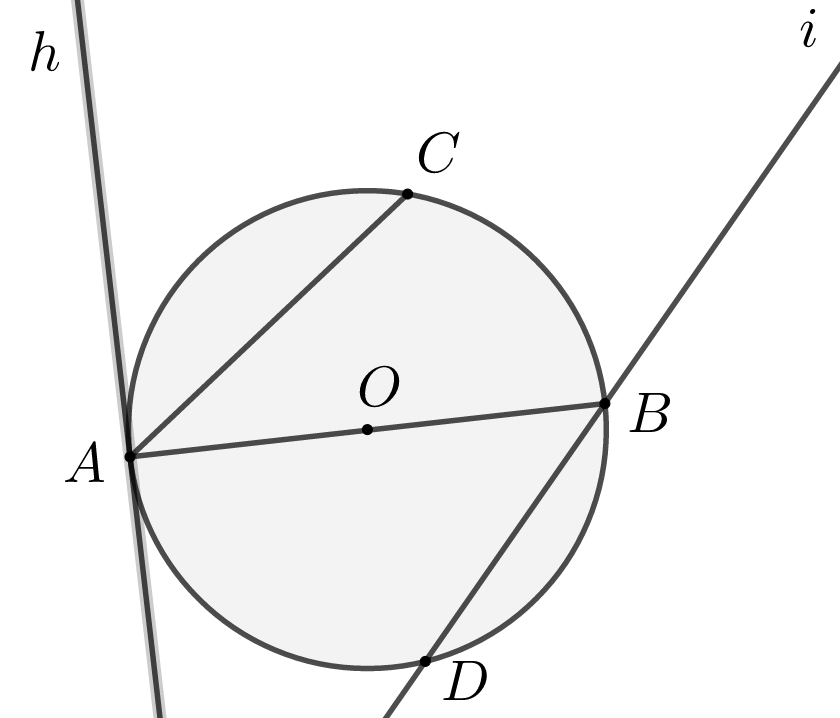
\includegraphics[width=0.3\textwidth]{Graphics/Week_13/GeometryDiagram.png}
		\label{fig: 2.1}
	\end{figure}
\end{frame}

\begin{frame}{Terminology}
\begin{itemize}
	\item Tangent (Line $h$): a line which touches the circle at only one point
	\item Secant (Line $i$): a line which passes through the circle, intersecting the circle at two points
	\item Arc ($\arc{BD}$): a part of the curve of the circle
\end{itemize}

\begin{figure}[h!]
	\centering
	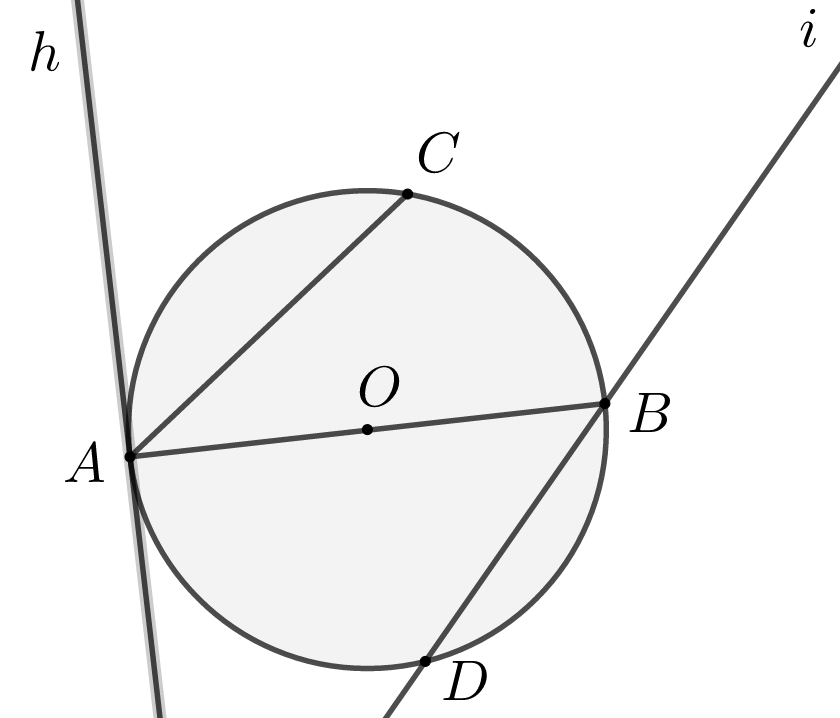
\includegraphics[width=0.3\textwidth]{Graphics/Week_13/GeometryDiagram.png}
	\label{fig: 2.1}
\end{figure}
\end{frame}

\section{Theorems}
\begin{frame}{Basic Formulas and Concepts}
\subsection{Basic Formulas and Concepts}
\begin{itemize}
	\item If $d$ is the diameter of the circle, and $r$ is the  radius of the circle, $d = 2r$
    \item The area of the circle, denoted $A$, is $A = \pi r^2$
    \itme The circumference of a circle, denoted $C$, is $C = \pi d = 2\pi r$
    \item The length of an arc, denoted $S$, is $S = r\theta$, where $\theta$ is the angle between the end points of the arc, in radians
\end{itemize}
\end{frame}

\subsection{Angle at the Center Theorem}
\begin{frame}{Angle at the Center Theorem}
The center angle subtended by any arc is twice any inscribed angle on that same arc. $\angle AOB = 2\angle ACB$


\begin{figure}[h!]
	\centering
	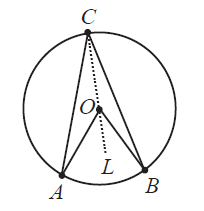
\includegraphics[height=0.4\textheight]{Graphics/Week_13/StarTreck.png}
\end{figure}
\end{frame}

\subsection{Thales' Theorem}
\begin{frame}{Thales' Theorem}
If a triangle is inscribed in a circle, where one side of the triangle is the diameter of the circle, then the angle opposite to that side is a right angle

\begin{figure}[h!]
	\centering
	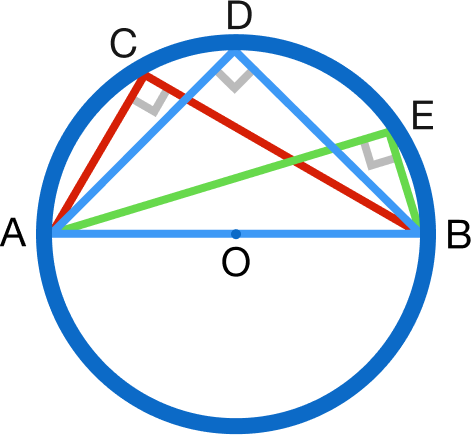
\includegraphics[height=0.4\textheight]{Graphics/Week_13/ThalesTheorem.png}
\end{figure}
\end{frame}

\subsection{Inscribed Angles}
\begin{frame}{Inscribed Angles}
The angles in the same segment from a common chord are equal.\\
$\angle ACB = \angle ADB = \frac{1}{2}\angle AOB$

\begin{figure}[h!]
	\centering
	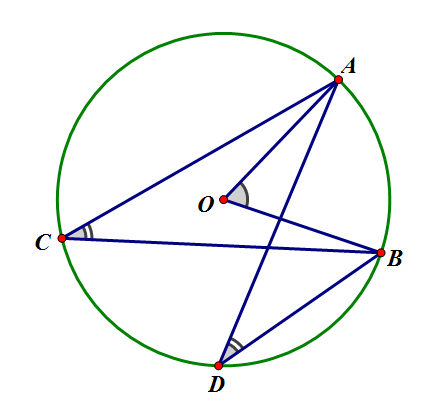
\includegraphics[height=0.5\textheight]{Graphics/Week_13/InscribedAngles.png}
\end{figure}
\end{frame}

\subsection{Intersecting Chords}
\begin{frame}{Intersecting Chords}
If two chords inside a circle intersect, the products of the intercepts of two intersecting chords are equal. $PA \cdot PB = PC \cdot PD$

\begin{figure}[h!]
	\centering
	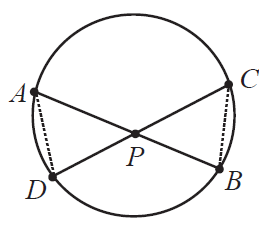
\includegraphics[height=0.5\textheight]{Graphics/Week_13/IntersectingChords.png}
\end{figure}
\end{frame}

\subsection{Alternate Segment Theorem}
\begin{frame}{Alternate Segment Theorem}
The angle between a tangent and a chord through the point of intersection is equal to the angle in the alternate segment. $\angle DCE = \angle DEB$

\begin{figure}[h!]
	\centering
	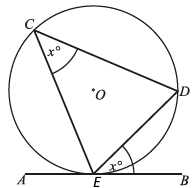
\includegraphics[height=0.5\textheight]{Graphics/Week_13/AlternateSegment.png}
\end{figure}
\end{frame}


\subsection{Tangent Angle Theorem}
\begin{frame}{Tangent Angle Theorem}
The tangent to a circle is perpendicular to the radius drawn to the point of intersection. $\angle OBC = 90^{\circ}$

\begin{figure}[h!]
	\centering
	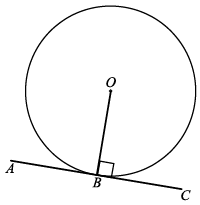
\includegraphics[height=0.5\textheight]{Graphics/Week_13/RightAngleTangent.png}
\end{figure}
\end{frame}

\subsection{Equal Tangent Theorem}
\begin{frame}{Equal Tangent Theorem}
Tangents to a circle from an external point of are equal. $AC = AB$

\begin{figure}[h!]
	\centering
	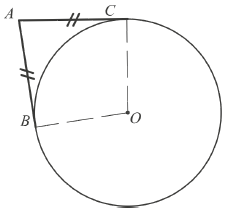
\includegraphics[height=0.5\textheight]{Graphics/Week_13/EqualTangents.png}
\end{figure}
\end{frame}

\subsection{Other Theorems (Perpendicular, Midpoint and Bisect Chords)}
\begin{frame}{Other Theorems (Perpendicular, Midpoint and Bisect Chords)}
If one of the following statements are true, then the other two statements are also true:
\begin{enumerate}
    \item The perpendicular from the center of a circle to a chord bisects the chord
    \item The line from the center of a circle of to the midpoint of a chord is perpendicular to the chord
    \item The perpendicular bisector of a chord passes through the center of the circle
\end{enumerate}

\begin{figure}[h!]
	\centering
	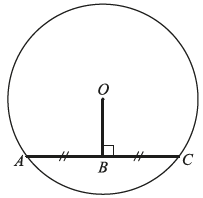
\includegraphics[height=0.3\textheight]{Graphics/Week_13/MidBisectChord.png}
\end{figure}
\end{frame}

\end{document}
